\documentclass{beamer}

\usetheme{Warsaw}
%\usetheme{CambridgeUS}

% modification history
% created on 18 sep 2011
% modified on 25 mar

%\usepackage{amsfonts, amsmath, amssymb}

%\setbeamertemplate{theorems}[numbered]
%\setbeamertemplate{theorems}[ams style] 
\usepackage[skins,breakable]{tcolorbox}
%\usepackage[normalem]{ulem}

%\usefonttheme[onlymath]{serif}                     // change the style of math font 

%=============set slide number=================
\addtobeamertemplate{navigation symbols}{}{
    \usebeamerfont{footline}
    \usebeamercolor[fg]{footline}
    \hspace{1em}
    \insertframenumber/\inserttotalframenumber
}
\setbeamercolor{footline}{fg=black}
\setbeamerfont{footline}{series=\bfseries}


%=============set footline=====================
\setbeamertemplate{footline}
{
  \leavevmode%
  \hbox{%
  \begin{beamercolorbox}[wd=.55\paperwidth,ht=2.25ex,dp=1ex,center]{author in head/foot}%
    \usebeamerfont{author in head/foot}\insertshortauthor
  \end{beamercolorbox}%
  \begin{beamercolorbox}[wd=.45\paperwidth,ht=2.25ex,dp=1ex,center]{title in head/foot}%
    \usebeamerfont{title in head/foot}\insertshorttitle
  \end{beamercolorbox}}%
  \vskip0pt%
}

%creating a rectangle box def
\newtcbox{\mybox}[1][red]{arc=0pt,outer arc=0pt,colback=#1!10!white,colframe=#1!50!black, boxsep=0pt,left=1pt,right=1pt,top=2pt,bottom=2pt,boxrule=0pt,bottomrule=1pt,toprule=1pt}

\newtcbox{\xmybox}[1][red]{arc=7pt,colback=#1!10!white,colframe=#1!50!black,before upper={\rule[-3pt]{0pt}{10pt}},boxrule=1pt,boxsep=0pt,left=6pt,right=6pt,top=2pt,bottom=2pt}
%the ``on line'' option doesn't work. so omitting it

%===== spacing =====

\def\extraspacing{\vspace{2mm} \noindent}
\def\vgap{\vspace{2mm}}
\def\hgap{\textrm{\hspace{1mm}}}

%===== tabbing =====

\def\tab{\hspace{2mm}}
\def\tabpos{\hspace{4mm} \= \hspace{4mm} \= \hspace{4mm} \= \hspace{4mm} \=
\hspace{4mm} \= \hspace{4mm} \= \hspace{4mm} \= \hspace{4mm} \= \hspace{4mm}
\kill}
\newcommand{\mytab}[1]{\begin{tabbing}\tabpos #1\end{tabbing}}

%===== blocks =====

% \newtheorem{theorem}{Theorem}
% \newtheorem{lemma}{Lemma}
% \newtheorem{corollary}{Corollary}
% \newtheorem{proposition}{Proposition}
% \newtheorem{definition}{Definition}
% \newtheorem{problem}{Problem}

\newcommand{\cbox}[2]{\begin{tcolorbox}[arc=0mm, colframe=#1!50!black, colback=#1!10!white]#2\end{tcolorbox}}
\newcommand{\minipg}[2]{\begin{center}\begin{minipage}{#1}#2\end{minipage}\end{center}}
\newcommand{\myfrm}[1]{\begin{frame}\begin{small}#1\end{small}\end{frame}} 
\newcommand{\myitems}[1]{\begin{itemize}#1\end{itemize}}
\newcommand{\myenums}[1]{\begin{enumerate}#1\end{enumerate}}
\newcommand{\myfig}[1]{\begin{figure}\centering #1\end{figure}}
    
%===== math macros =====
\newcommand{\bm}[1]{\textrm{\boldmath${#1}$}}
%\newcommand{\smat}[2]{\left[\begin{tabular}{#1}#2\end{tabular}\right]}
%\newcommand{\bmat}[2]{\left|\begin{tabular}{#1}#2\end{tabular}\right|}
\newcommand{\bmat}[1]{\begin{bmatrix}#1\end{bmatrix}}
\newcommand{\vmat}[1]{\begin{vmatrix}#1\end{vmatrix}}
\newcommand{\myeqn}[1]{\begin{eqnarray}#1\end{eqnarray}}
\newcommand{\set}[1]{\{#1\}}

\def\eps{\epsilon}
\def\fr{\frac}
\def\lc{\lceil}
\def\lf{\lfloor}
\def\rc{\rceil}
\def\rf{\rfloor}
\def\Pr{\textrm{\boldmath$Pr$}}
\def\expt{\textrm{\boldmath$E$}}
\def\real{\mathbb{R}}
\def\int{\mathbb{Z}}
\def\*{\star}
\def\tO{\tilde{O}}

\DeclareMathOperator*{\argmin}{arg\,min}
\DeclareMathOperator*{\polylg}{polylg}
\DeclareMathOperator*{\polylog}{polylog}
\DeclareMathOperator*{\intr}{\cap}

\def\nn{\nonumber}
\def\mit{\mathit}


%===== misc =====

\def\done{\hspace*{\fill} $\framebox[2mm]{}$}	% end of proof
\def\ttt{\texttt}

%===== coloring =====
\newcommand{\red}[1]{\textcolor{red}{#1}}
\newcommand{\bred}[1]{\textcolor{red}{\bf #1}}
\newcommand{\blue}[1]{\textcolor{blue}{\bf #1}}

\usepackage{color}
\usepackage{graphicx}
\usepackage{multirow}
\usepackage[skins,breakable]{tcolorbox}

\def\done{\hfill$\square$}
\def\vgap{\vspace{5mm}}


\title{Small and Sweet MapReduce Algorithms}

\author{Yufei Tao}
\institute[]
{Chinese University of Hong Kong}
\date{}

\begin{document}
%-------------------------------------------------------------
\begin{frame}
\titlepage
\end{frame}
%-------------------------------------------------------------
\begin{frame}
\begin{small}
    \xmybox{MapReduce}
    
    \vgap 
    
    A platform for massive parallel computation. 
    
    \begin{itemize} 
        \item First (formal) paper in 2004. 
        \item Now a large collection of algorithms on this platform.  
    \end{itemize}
\end{small}
\end{frame}
%-------------------------------------------------------------
\begin{frame}
\begin{small}
    %\xmybox{MapReduce}
    
    \vgap 
    
    \begin{tcolorbox}[arc=0mm, colframe=green!50!black, colback=green!10!white] 
        \blue{This talk:} \\
        \red{Principles} in the design and analysis of algorithms in MapReduce (and other similar platforms).
    \end{tcolorbox} 
    
    \vgap
    \pause 
    
    Ultimate goals:
    \begin{itemize} 
        \item \red{Small:} Simple enough for practical implementation 
        \item \red{Sweet:} With non-trivial theoretical guarantees. 
    \end{itemize}


\end{small}
\end{frame}
%-------------------------------------------------------------
\begin{frame}
\begin{small}
    \xmybox{Computation Model}
    
    \vgap 

    This is the starting point before any meaningful analysis.
    
    \vgap
    
    \begin{tcolorbox}[arc=0mm, colframe=blue!50!black, colback=blue!10!white] 
        \begin{enumerate} 
            \item[1.] MRC model [SODA'10]  
            \item[2.] BSP-like model [ISSAC'11]
        \end{enumerate}
    \end{tcolorbox}
    
        
    \begin{tcolorbox}[arc=0mm, colframe=green!50!black, colback=green!10!white] 
        \begin{enumerate}
        \item[3.] \red{Minimality Model} [SIGMOD'13] 
        \item[4.] \red{Massively Parallel Computation} (MPC) [PODS'13]. 
        \end{enumerate}
    \end{tcolorbox}
    
\end{small}
\end{frame}
%-------------------------------------------------------------
\begin{frame}
\begin{small}
    \xmybox{Computation Model}
    
    \vgap 

    This talk:
    
    \vgap
        
    \begin{tcolorbox}[arc=0mm, colframe=green!50!black, colback=green!10!white] 
        \begin{enumerate}
        \item[3.] \red{Minimality Model} [SIGMOD'13] 
        \begin{itemize} 
            \item A very stringent model -- suitable for studying ``easy'' problems.
        \end{itemize}

        \item[4.] \red{Massively Parallel Computation} (MPC) [PODS'13]. 
        \begin{itemize} 
            \item A more relaxed model -- suitable for studying ``hard'' problems.
        \end{itemize}

        \end{enumerate}
    \end{tcolorbox}
    
\end{small}
\end{frame}
%-------------------------------------------------------------
\begin{frame}
\begin{small}
    \xmybox{Minimality Model}
    \vgap
    %\begin{center}
    \mybox[green]{Input and Machines} 
    %\end{center}
    
    \vgap 

    \red{$p$} = number of machines. \\ 
    \red{$n$} = number of elements in the input (i.e., dataset) \\
    Assumption: \red{$p \le \sqrt{\fr{n }{2 \ln n}}$}
    
    \vgap 
    
    At the beginning, $\red{O(n / p)}$ elements per machine. 
    \begin{itemize} 
        \item The algorithm has no control over how the elements are initially distributed.
    \end{itemize}

    
\end{small}
\end{frame}
%-------------------------------------------------------------
\begin{frame}
\begin{small}
    \xmybox{Minimality Model}
    
    \vgap
    %\begin{center}
    \mybox[green]{Superstep} 
    %\end{center}
    
    %\vgap
    
    Two phases: 
    
    \begin{enumerate} 
        \item Machines message each other. 
        \pause
%         \begin{itemize} 
%             \item Constraint 1: Every machine can \red{send $O(n/p)$} words only. 
%             \item Constraint 2: Every machine can \red{receive $O(n/p)$} words only. 
%         \end{itemize} 
        
        \item Machines perform local computation (all operations in the RAM model allowed). 
        
    \end{enumerate}

    \vgap
    \pause
    \mybox[green]{Algorithm} 
   
    %\vgap
    An \red{algorithm} is a sequence of supersteps. 
    
    
\end{small}
\end{frame}
%-------------------------------------------------------------
\begin{frame}
\begin{small}
    \xmybox{Minimality Model}
    
    \vgap 
    
    Consider a computational problem \red{$\Pi$}. Suppose that it can be solved in \red{$f(n) = \Omega(n)$} time \red{sequentially} in the RAM model. 
    
    \pause
    
    \vgap 
    
    \begin{tcolorbox}[arc=0mm, colframe=blue!50!black, colback=blue!10!white] 
    $\Pi$ is \red{minimal} if it admits an algorithm satisfying all:  
    \begin{enumerate} 
        \item It has \red{$O(1)$} supersteps. 
        \item It uses \red{$O(n/p)$} space at all times.
        \item Every machine sends \red{$O(n/p)$} words in total. 
        \item Every machine incurs \red{$O(f(n/p))$} CPU time in total. 
%         \begin{itemize} 
%             \item[] \xmybox[red]{Must improve whenever $f(n)$ is improved!}
%         \end{itemize}
%   
    \end{enumerate}
    \vgap
    The algorithm is called a \red{minimal algorithm} for $\Pi$.
    \end{tcolorbox} 
    
%      
%     
%     \vgap
% 
%     Next, let us look at each criterion in turn, and understand why the name ``minimal''. 
\end{small}
\end{frame}
%-------------------------------------------------------------
\begin{frame}
\begin{small}
    \xmybox{Minimality Model}
    
    \vgap 
    
    \blue{Requirement 1: $O(1)$ supersteps.}
    
    \pause
    \vgap
    
    \blue{Requirement 2: $O(n/p)$ space at all times.} 
    
    Balanced during the entire algorithm. 
    
    \pause
    \vgap
    
    \blue{Requirement 3: $O(n/p)$ words sent and received.} 
    
    Asymptotically the same time for each machine to look at its portion of the input.
\end{small}
\end{frame}
%-------------------------------------------------------------
\begin{frame}
\begin{small}
    \xmybox{Minimality Model}
    
    \vgap 
    
    \blue{Requirement 4: $O(f(n/p))$ CPU time for every machine.}
    
    \begin{itemize} 
        \item The MapReduce algorithm \red{must improve automatically} whenever a faster sequential algorithm is discovered!
        \begin{itemize}
            \item Implies that the MapReduce algorithm must utilize a sequential algorithm as a \red{black box}!
        \end{itemize} 
        
        \vgap \pause
        
        \item The best you can do! 
        \begin{itemize}
            \item If you can achieve $o(f(n/p))$ on MapReduce, you can simulate the same algorithm in the RAM model in $o(p \cdot f(n/p))$ time. 
        \end{itemize} 
        
    \end{itemize}

    
\end{small}
\end{frame}
%-------------------------------------------------------------
\begin{frame}
\begin{small}
    \xmybox{Minimal Algorithm for Sorting}
    
    \vgap 
    
    \blue{At the beginning:} $n$ elements on $p$ machines. \\
    \blue{At the end:} it is possible to label the machines from 1 to $p$ such that all elements on machine $i$ are smaller than those on machine $j$, for any $i < j$. 
    
    
    \vgap \vgap \pause
    
    \begin{tcolorbox}[arc=0mm, colframe=blue!50!black, colback=blue!10!white] 
        \red{Remark (illustration of Requirement 4)} 
        \begin{itemize} 
            \item Comparison-based sort: $\Theta(n \log n)$ sequentially $\Rightarrow$ $O(\fr{n}{p} \log \fr{n}{p})$ MapReduce . 
            \item Sorting $n$ integers: $O(n \log\log n)$ sequentially $\Rightarrow$ $O(\fr{n}{p} \log\log \fr{n}{p})$ MapReduce. 
        \end{itemize}
        
        All by the same algorithm. 
    \end{tcolorbox}

    
    
\end{small}
\end{frame}
%-------------------------------------------------------------
\begin{frame}
\begin{small}
    \xmybox{Minimal Algorithm for Sorting}
    
    \vgap 
    
    \mybox[green]{Superstep 1} 
    
    
    \begin{itemize} 
        \item \blue{Phase 1:} Each machine samples each object with probability \red{$\rho = \fr{p}{n} \ln (np)$} independently, and sends the samples to all other machines. 
        
        \item \blue{Phase 2:} Each machine sorts the samples received, and identify the \red{split elements} that partition the list into $t$ segments evenly.  
        \begin{itemize} 
            \item Machine $i$ will get all the elements in the $i$-th segment at the end.
        \end{itemize} 
    \end{itemize}

    \vgap
        
    \begin{center} 
        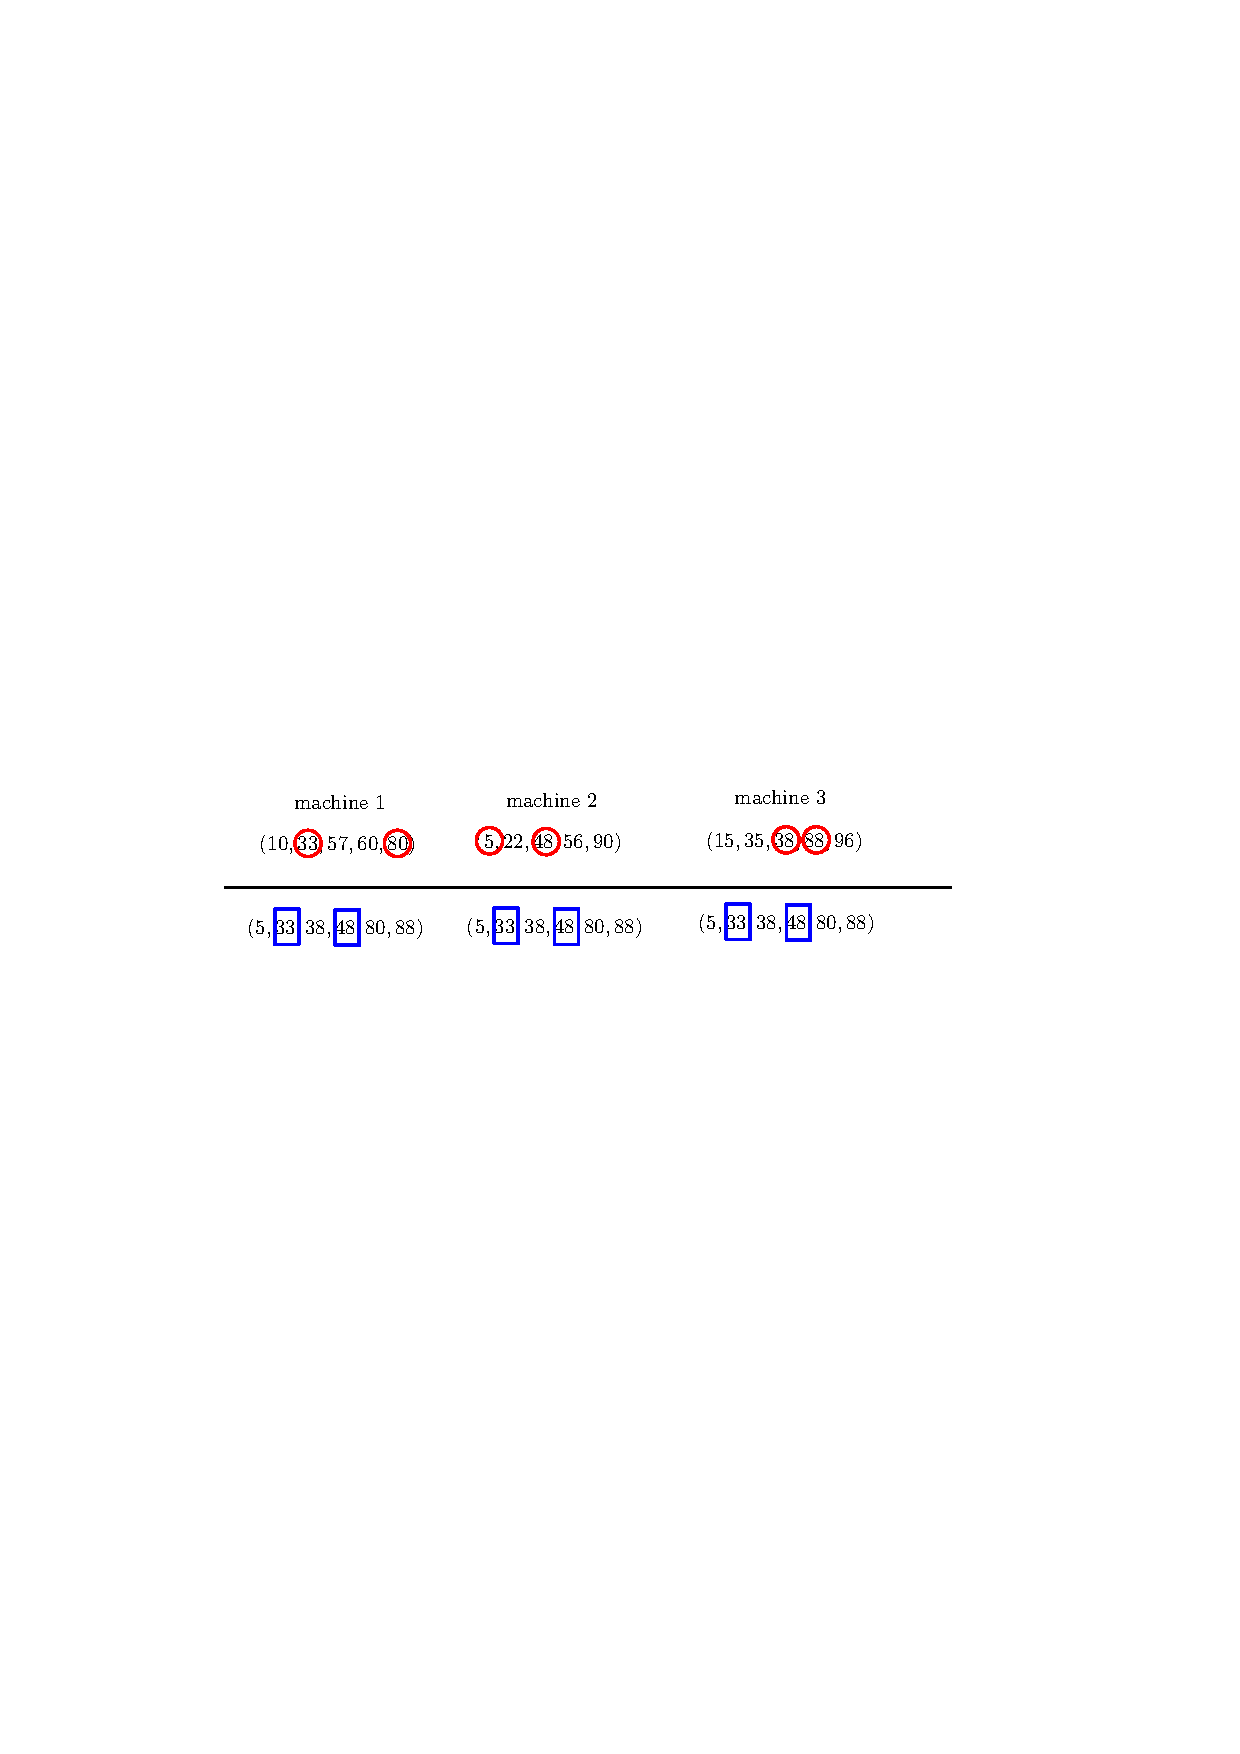
\includegraphics[height=20mm]{./artwork/tera} 
    \end{center}
\end{small}
\end{frame}
%-------------------------------------------------------------

\begin{frame}
\begin{small}
    \xmybox{Minimal Algorithm for Sorting}
    
    \vgap 
    
    \mybox[green]{Superstep 2} 
    
    
    \begin{itemize} 
        \item \blue{Phase 1:} Each machines sends the elements in the $i$-th segment to machine $i$. 
        
        \item \blue{Phase 2:} Machine $i$ sorts the elements in the $i$-th segment.
    \end{itemize}

    \begin{center} 
        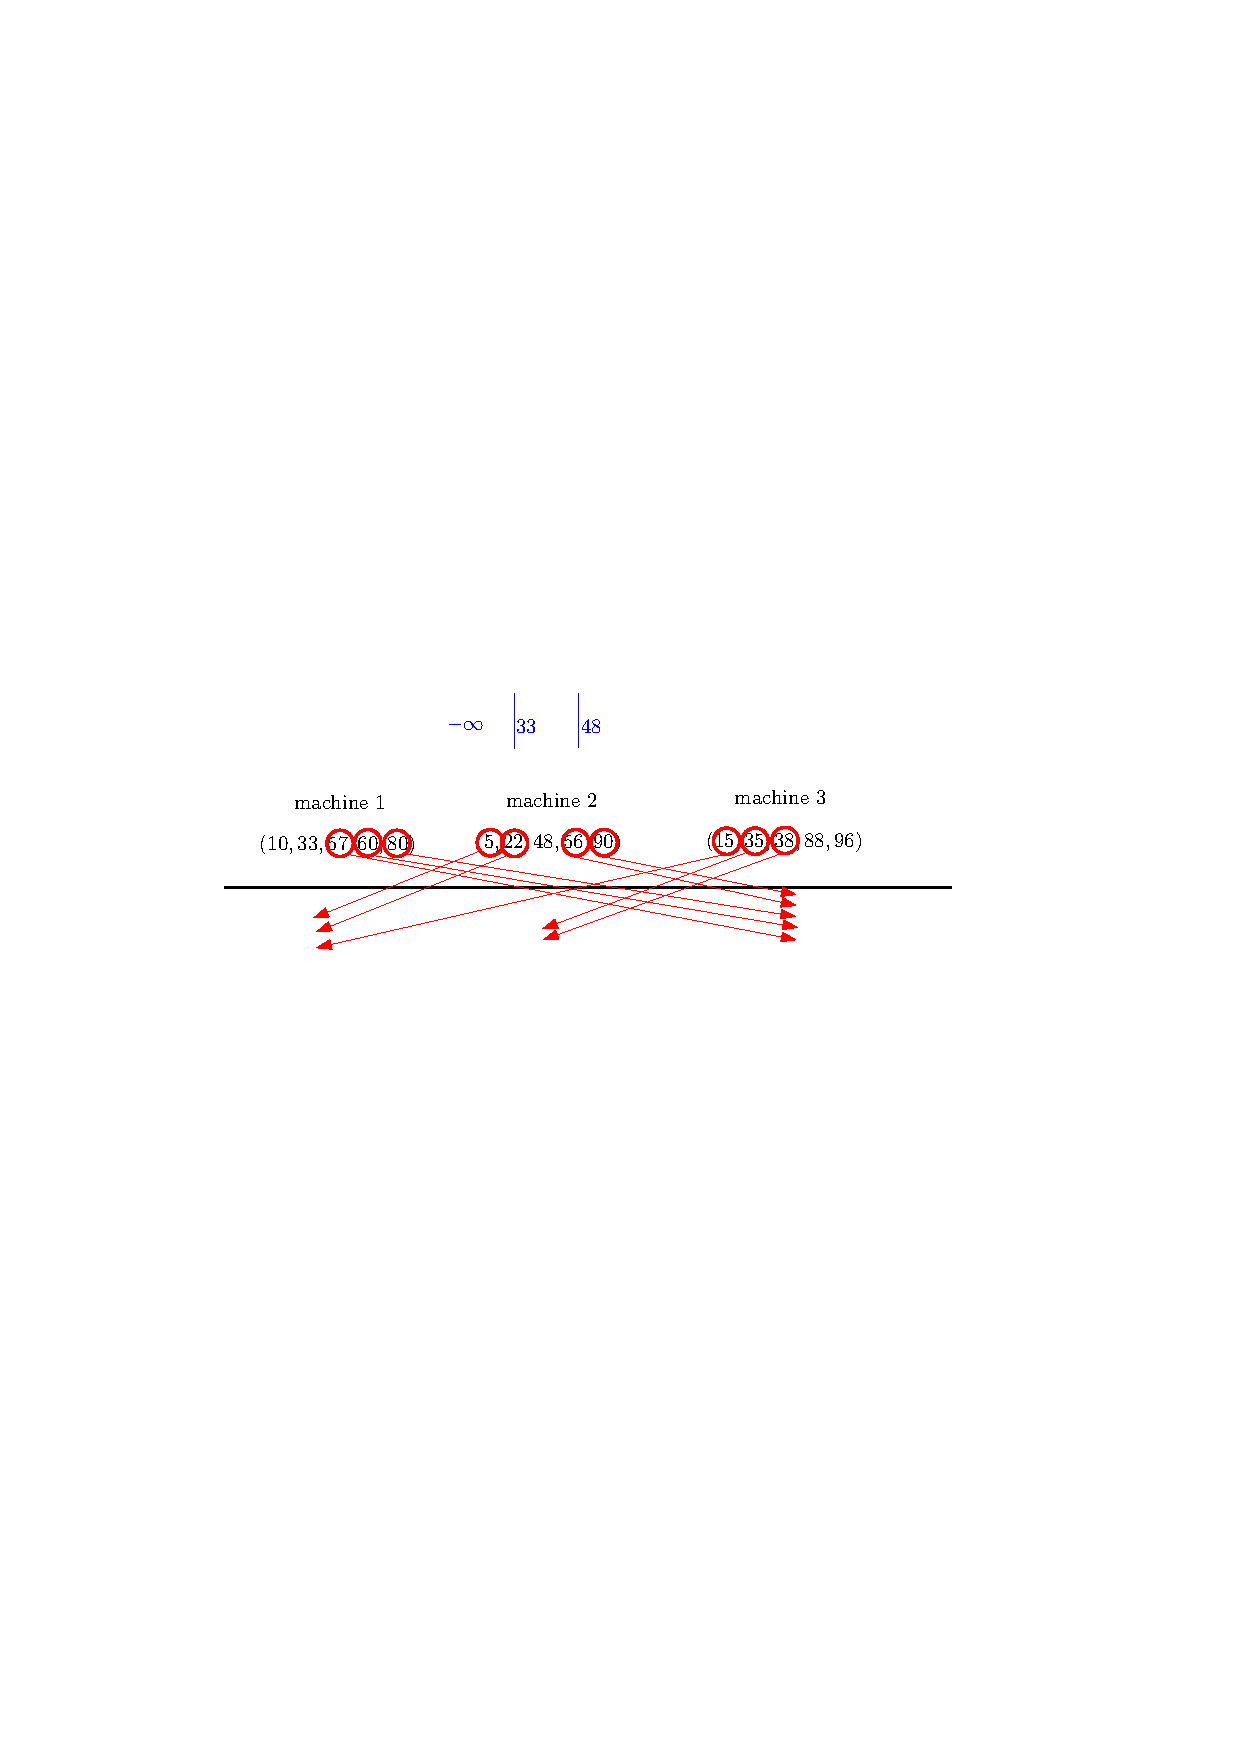
\includegraphics[height=35mm]{./artwork/tera1} 
    \end{center}
\end{small}
\end{frame}
%-------------------------------------------------------------
\begin{frame}
\begin{small}
    \xmybox{Minimal Algorithm for Sorting}
    
    \vgap 
    
    \blue{Theorem:} The above algorithm is minimal with probability at least $1 - O(1/n)$. 
    
    \vgap \vgap 
    
    
\end{small}
\end{frame}
%-------------------------------------------------------------
\begin{frame}
\begin{small}
    \xmybox{Minimality $\Rightarrow$ MPC}
    
    \vgap 
        
    For certain problems, if $O(1)$ supersteps are required, it is impossible to ensure that each machine sends $O(n/p)$ words only. \\
    $\Rightarrow$ \red{No minimal algorithms}. 
    
    
    \vgap \pause
    
    Phrased differently, if $O(1)$ supersteps are required, we must allow a machine to send more than $O(n/p)$ words -- but how much more? \\
    $\Rightarrow$ \red{The MPC model}. 
\end{small}
\end{frame}
%-------------------------------------------------------------
\begin{frame}
\begin{small}
    \xmybox{MPC Model}
    \vgap
    %\begin{center}
    \mybox[green]{Input and Machines} 
    %\end{center}
    
    \vgap 

    \red{$p$} = number of machines. \\ 
    \red{$n$} = number of elements in the input (i.e., dataset) \\
    Assumption: \red{$p \le n^{1/c}$ for some constant $c > 1$.}
    
    \vgap 
    
    At the beginning, $\red{O(n / p)}$ elements per machine. 
    \begin{itemize} 
        \item The algorithm has no control over how the elements are initially distributed.
    \end{itemize}

    
\end{small}
\end{frame}
%-------------------------------------------------------------
\begin{frame}
\begin{small}
    \xmybox{MPC Model}
    
    \vgap
    %\begin{center}
    \mybox[green]{Superstep} 
    %\end{center}
    
    %\vgap
    
    Two phases: 
    
    \begin{enumerate} 
        \item Machines message each other. 
%         \begin{itemize} 
%             \item Constraint 1: Every machine can \red{send $O(n/p)$} words only. 
%             \item Constraint 2: Every machine can \red{receive $O(n/p)$} words only. 
%         \end{itemize} 
        
        \item Machines perform local computation (all operations in the RAM model allowed). 
        
    \end{enumerate}

    \vgap
    \mybox[green]{Algorithm} 
   
    %\vgap
    An \red{algorithm} is a sequence of supersteps. 
    
    
\end{small}
\end{frame}
%-------------------------------------------------------------
\begin{frame}
\begin{small}
    \xmybox{MPC Model}
    
    \vgap 
    
    An algorithm is required to finish in $O(1)$ supersteps. 
    
    \vgap \pause 
    
    \red{Communication cost of one machine} = \\
    Total number of words it communicated (sent and received combined) 
    
    \vgap \pause
    
    \red{Load} of the algorithm =  \\
    Communication cost of the most expensive machine 
    
    \vgap \pause 
    
    Aim: Minimize load. 
    
    \vgap \pause
    
    \begin{tcolorbox}[arc=0mm, colframe=blue!50!black, colback=blue!10!white] 
        \blue{Remark 1:} CPU time for free. \\ \pause 
        \blue{Remark 2:} Every minimal algorithm must have load $O(n/p)$. \\ \pause
        \blue{Remark 3:} Any problem admits an algorithm of load $O(n)$. 
    \end{tcolorbox}

\end{small}
\end{frame}
%-------------------------------------------------------------
\begin{frame}
\begin{small}
    \xmybox{MPC Model}
    
    \vgap 
    
    The MPC model has largely been used to study problems where the output size can be much larger than $n$, e.g., joins. 
    
    \vgap \pause 
    
    Focus of this talk: \blue{Cartesian Product} \pause
    
    \vgap
    
    \red{$R$:} a set of \red{$n$} \red{\bf red} elements \\ 
    \red{$S$:} a set of \red{$n$} \blue{blue} elements \\ 

    \vgap 
    
    \blue{At the beginning:} The $2n$ elements are stored on the $p$ machines (each $O(n/p)$ elements). \\ 
    \blue{At the end:} Each element in $R \times S$ must appear on some machine. 
\end{small}
\end{frame}
%-------------------------------------------------------------
\begin{frame}
\begin{small}
    \xmybox{MPC Lower Bound for Cartesian Product}
    
    \vgap 
    
    To warm up, we will prove that, when $p = 2$, any algorithm solving the problem must have load $\red{\Omega(n)}$. 
    
    \vgap
    
    \red{$\Rightarrow$ Implication:} No better algorithm than simply sending everything over to the other machine.  
    
    
    
\end{small}
\end{frame}
%-------------------------------------------------------------
% \begin{frame}
% \begin{small}
%     \xmybox{MPC Lower Bound for Cartesian Product}
%     
%     \vgap 
%     
%     
%     Suppose that machine 1 has \red{$c_1 n$} red and \blue{$c_2 n$} blue elements for constants $0\le c_1, c_2 \le 1$. \\
%     $\Rightarrow$ Machine 2 has has \red{$(1 - c_1) n$} red and \blue{$(1 - c_2) n$} blue elements \\ 
%     
%     \vgap
%     
%     With no communication, the two machines can produce 
%     \begin{eqnarray} 
%         c_1 c_2 n^2 + (1 - c_1)(1 - c_2) n^2 \le n^2 / 2 \nn
%     \end{eqnarray}
%     pairs in the cartesian product. \\
%     $\Rightarrow$ Still $n^2 / 2$ pairs to produce. \\
%     $\Rightarrow$ At least $n^2 / \red{4}$ pairs produced on one machine -- say machine 1 \\ 
%     $\Rightarrow$ Machine 1 must get $$\fr{n^2 / 4}{\max\{c_1, c_2\} \cdot n} = \Omega(n)$$ elements from machine 2. \\ 
% \end{small}
% \end{frame}
% %-------------------------------------------------------------
\begin{frame}
\begin{small}
    \xmybox{MPC Lower Bound for Cartesian Product}
    
    \vgap 
    
    For simplicity, assume each machine has $n$ elements at the beginning. 
    
    \vgap 
    
    
    Suppose that an algorithm solves the problem with load \red{$L$}. \\ \pause 
    $\Rightarrow$ Machine 1 sees \red{$n + L$} elements overall. \\ \pause
    $\Rightarrow$ It can produce at most $$\left(\fr{n + L}{2}\right)^2$$ pairs\\ \pause 
    $\Rightarrow$ Same for machine 2. \\ \pause 
    $\Rightarrow$ 
    \begin{eqnarray} 
        2 \left(\fr{n + L}{2}\right)^2 &\ge& n^2 \nn \pause
    \end{eqnarray}
    which solves to $L \ge \fr{2 - \sqrt{2}}{2\sqrt{2}} n$. 
\end{small}
\end{frame}
%-------------------------------------------------------------
\begin{frame}
\begin{small}
    \xmybox{MPC Lower Bound for Cartesian Product}
    
    \vgap 
    
    Next, we will extend the algorithm to prove that, any cartesian product algorithm must have load $\red{\Omega(n / \sqrt{p})}$. 
    
    \vgap
    
    \red{$\Rightarrow$ Implication:} No minimal algorithm!  
    
\end{small}
\end{frame}
%-------------------------------------------------------------
\begin{frame}
\begin{small}
    \xmybox{MPC Lower Bound for Cartesian Product}
    
    \vgap 
    
    
    Suppose that an algorithm has load \red{$L$}. \\ \pause 
    $\Rightarrow$ Every machine can receive at most $L$ elements. \\ \pause
    $\Rightarrow$ In total, the machine sees $\red{c \cdot n/p + L}$ elements during the entire algorithm. \\ \pause 
    $\Rightarrow$ The machine can produce at most 
    \begin{eqnarray} 
        \left(\fr{c \cdot n/p + L}{2} \right)^2 \nn
    \end{eqnarray}
    pairs. \\ \pause 
    $\Rightarrow$ Putting together $p$ machines means
    \begin{eqnarray} 
        p \cdot \left(\fr{c \cdot n/p + L}{2} \right)^2 &\ge& n^2 \nn \pause
    \end{eqnarray}
    which solves to $L = \Omega(n / \sqrt{p})$.
\end{small}
\end{frame}
%-------------------------------------------------------------
\begin{frame}
\begin{small}
    \xmybox{MPC Lower Bound for Pairwise Natural Join}
    
    \vgap 
    
    
    \blue{Pairwise Natural Join} 
    
    \vgap
    
    \red{$R = (A, B)$:} a table of \red{$n$} tuples \\ 
    \red{$S = (B, C)$:} a table of \red{$n$} tuples \\ 

    \vgap 
    
    \blue{At the beginning:} The $2n$ tuples are stored on the $p$ machines. \\ 
    \blue{At the end:} Each element in $R \bowtie S$ must appear on some machine. 
    
    \vgap \vgap \pause
    
    \blue{LOWER BOUND:} Load $\Omega(n/\sqrt{p})$! 
\end{small}
\end{frame}
%-------------------------------------------------------------
\begin{frame}
\begin{small}
    \xmybox{MPC Cartesian Product}
    
    \vgap 
    
    
    An optimal algorithm---named \red{cube}---with load $O(n/\sqrt{p})$ is known.  \\
    The algorithm actually computes the cartesian product. \\
    
    \begin{center} 
        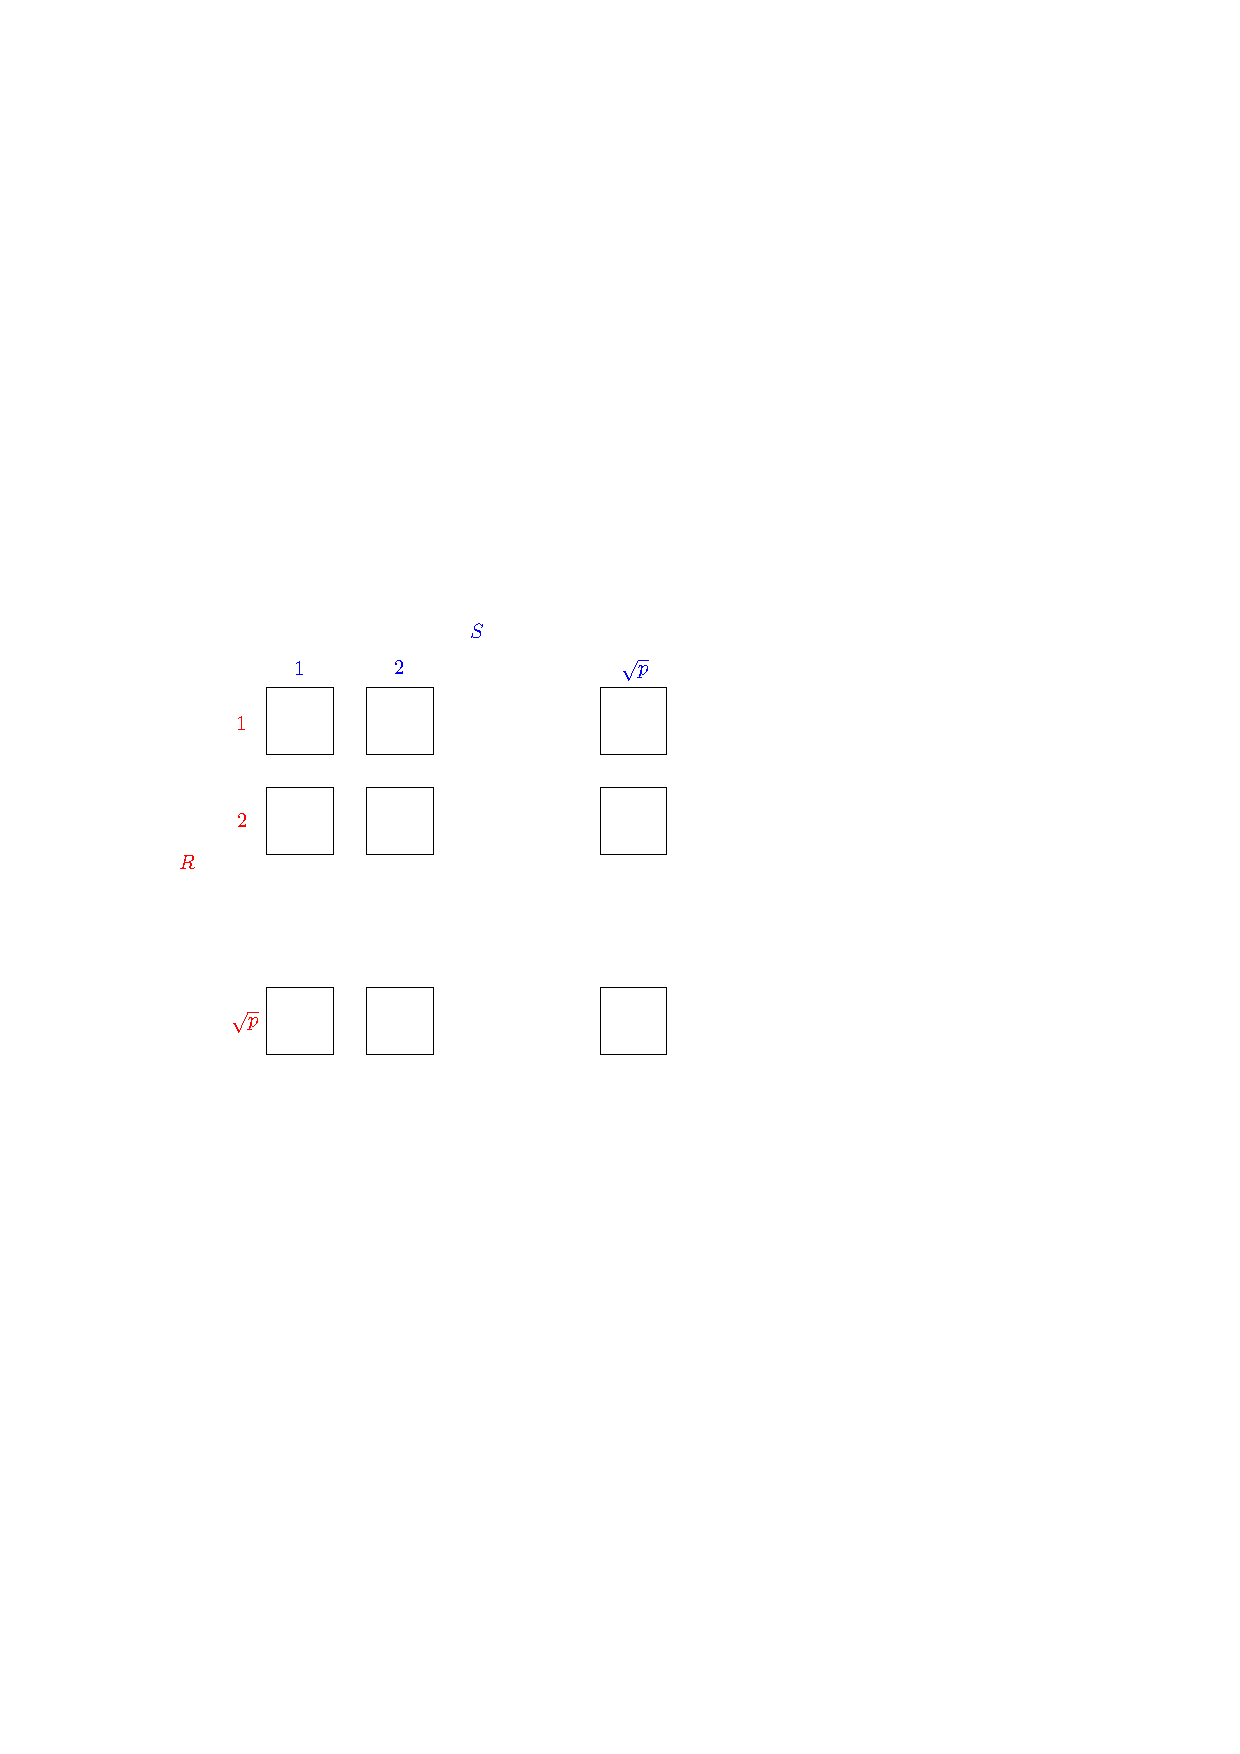
\includegraphics[height=50mm]{./artwork/cube}
    \end{center}

    
\end{small}
\end{frame}
%-------------------------------------------------------------
\begin{frame}
\begin{small}
    \xmybox{MPC Model: Understood Problems}
    
    \vgap 
    
    
    Problems whose communication complexities (i.e., load) have been well understood: 
    
    \begin{itemize} 
        \item Enumeration of constant-sized subgraphs.
        \item Restricted natural joins. 
        \item Linear programming. 
        \item ...
    \end{itemize}


    
\end{small}
\end{frame}
%-------------------------------------------------------------
\begin{frame}
\begin{small}
    \xmybox{Summary}
    
    \vgap 
    
    
    \red{Principles} in design and analysis of MapReduce algorithms 
    \begin{itemize} 
        \item Minimality 
        \item MPC
    \end{itemize}

    
    \vgap \pause
    
    Future work 1: Re-examine \red{all} problems! \\ \pause
    Future work 2: Lower bound for problems with \red{small} result sizes! 
    \begin{itemize} 
        \item From the theory of communication complexity, it is easy to prove that when $p = 2$, $\Omega(n)$ communication is necessary for detecting whether a natural join has an empty result! \pause
    \end{itemize}
    Future work 3: $o(n/p)$-load algorithms! 
    
\end{small}
\end{frame}
%-------------------------------------------------------------

\end{document}  

%17095162812
